

\section{Klärung der Begrifflichkeiten}

\subsection{BMK-IoT Modul}
Das „BMK-IoT Modul“ ist ein Design In Modul. Eine bereits entwickelte Hardwaregrundlage mit Mikrocontroller, WLAN-Chip, eMMC und weiteren Schnittstellen, sowie fertigen Softwaregrundlagen im Bereich der Embedded Security, RTOS und Cloud ermöglichen der BMK-Entwicklung kundenspezifische Projekte schneller und einheitlicher zu realisieren.
Die dafür benötigte Hardware findet auf einer kleinen Platine mit BGA-Sockel Platz. 

\begin{center}
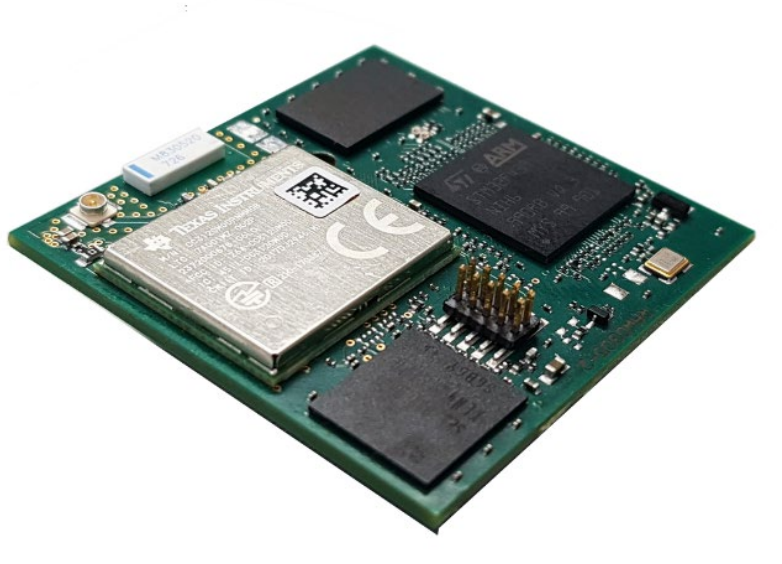
\includegraphics[width=10cm]{Bilder/BMK-IOT-MODUL.png}
\end{center}



\subsection{LaTeX}
LaTeX ist wie MS-Word oder Libre-Office ein Textverarbeitungsprogramm. Werden in einem klassischen Word.doc, Text und Grafik gleichzeitig erstellt und während des gesamten Erstellungsprozesses auf dem Monitor dargestellt, so werden unter Latex diese Bereiche separiert. Inhalt und Layout werden erst durch einen separaten Schritt in eine Ausgabedatei generiert. Über viele Jahre hinweg wurden durch eine große Community immer mehr Libraries, welche wissenschaftliche Standards etablierten veröffentlicht und können in ein LaTeX-Dokument sehr einfach importiert werden. Bei richtiger Einbindung der Libraries wird das Geschriebene von LaTeX automatisch in ein richtiges Layout gebracht. Aus diesem Grund ist LaTeX ein sehr beliebtes Tool, zum Verfassen von wissenschaftlichen Arbeiten.

\newpage
\subsection{Pig-Tail}
Um bei hohen Frequenzen mit einem Oszilloskop bessere Messergebnisse zu erhalten, ist es oft hilfreich, ein Pig-Tail zu verwenden. Diese können oft beim Hersteller gekauft oder mit Silberdraht selbst gewickelt werden. 
\\
Das Messergebnis verbessert sich durch die niedrigere Induktivität der Masseleitung. Das über bzw. unterschingen des Messsignales verringert sich dadurch sichtbar. 


\begin{center}

\includegraphics[width=10cm]{Bilder/PigTail.jpg}


\end{center}


\begin{figure}[htb]
    \centering
    \begin{minipage}[t]{0.45\linewidth}
        \centering
        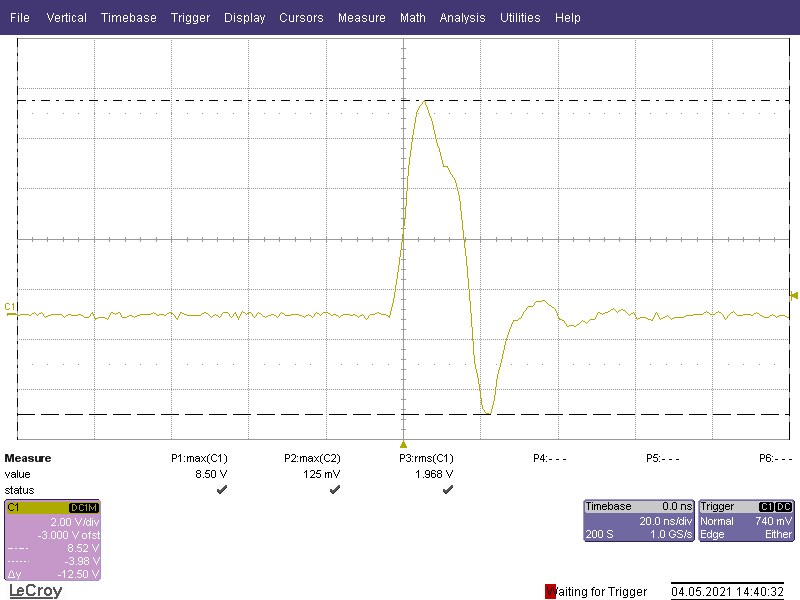
\includegraphics[width=8cm]{Bilder/TP19-ohne-PigTail.png}
        \caption{Signal ohne Pig-Tail}
    \end{minipage}% <- sonst wird hier ein Leerzeichen eingefügt
    \hfill
    \begin{minipage}[t]{0.45\linewidth}
        \centering
        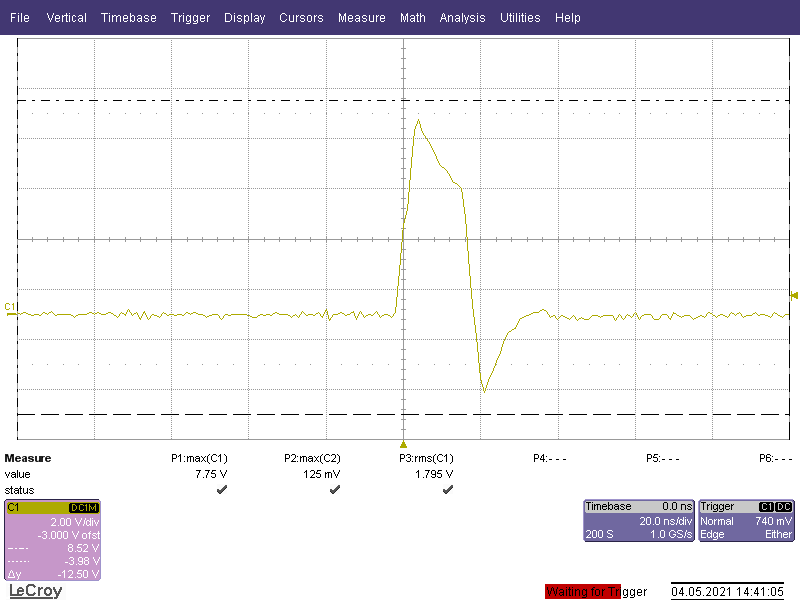
\includegraphics[width=8cm]{Bilder/TP19-mit-PigTail.png}
        \caption{Signal mit Pig-Tail}
    \end{minipage}
\end{figure}
